\documentclass[11pt,twocolumn,a4paper]{article}
\usepackage{amsmath}
\usepackage{amssymb}
\usepackage{graphicx}
\usepackage{booktabs}
\usepackage{hyperref}
\usepackage{float}
\usepackage{geometry}
\usepackage{xcolor}
\usepackage{microtype}
\usepackage{titlesec}
\usepackage{caption}
\usepackage{abstract}
\usepackage{fancyhdr}

% Page geometry matching Springer twocolumn style
\geometry{
    a4paper,
    left=15mm,
    right=15mm,
    top=22mm,
    bottom=22mm,
    footskip=10mm
}

\hypersetup{
    colorlinks=true,
    linkcolor=blue,
    filecolor=magenta,      
    urlcolor=cyan,
    pdftitle={Enhancing Geoheritage Evaluation in Morocco: A Nationwide Machine Learning-Based Geosite Accessibility Model under Spatial Block Cross-Validation},
    pdfpagemode=FullScreen,
}

\raggedbottom

% Set up headers and footers to resemble the journal page
\pagestyle{fancy}
\fancyhf{}
\fancyhead[L]{\textsf{GSMI-UM6P}}
\fancyhead[R]{\textsf{Internship Technical Report — Fuzzy MCDSS Model}}
\fancyfoot[C]{\thepage}
\renewcommand{\headrulewidth}{0.4pt}
\renewcommand{\footrulewidth}{0pt}

% Section formatting matching Springer
\titleformat{\section}{\large\bfseries\sffamily}{\thesection}{1em}{}
\titleformat{\subsection}{\normalsize\bfseries\sffamily}{\thesubsection}{1em}{}

% Redefine abstract style
\renewenvironment{abstract}{%
    \small\sffamily
    \noindent\textbf{Abstract}\quad
}{%
    \vspace{0.4cm}
}

\begin{document}

% GSMI Header on first page
\twocolumn[
    \begin{@twocolumnfalse}
        \begin{center}
            {
\includegraphics[width=0.45\textwidth]{../um6p_figures/um6p_gsmi_logo.png}}
        \end{center}
        \vspace{0.4cm}
        
        {\Huge\bfseries\sffamily Enhancing Geoheritage Evaluation in Morocco: A Nationwide Machine Learning-Based Geosite Accessibility Model under Spatial Block Cross-Validation\par}
        \vspace{0.6cm}
        
        {\large\textbf{EL GORRIM Mohamed}\par}
        {\small\sffamily AI Research Intern, Geology and Sustainable Mining Institute (GSMI), Mohammed VI Polytechnic University (UM6P), Ben Guerir, Morocco\par}
        \vspace{0.4cm}
        {\small\sffamily\textbf{Prepared for:} Dr. Ismail BEN AMAR, Sanae EL HARCHE, and Mohamed EL OUALI\par}
        \vspace{0.6cm}
        
        \begin{abstract}
        Assessing the accessibility of geological heritage sites (geosites) across large territories is critical for sustainable geotourism and conservation planning. Building upon the localized machine learning (ML) framework established by Naimi et al. (2025) for the Ziz Upper Watershed, this work presents a comprehensive, nationwide scaling of geosite modeling to the entire territory of Morocco. We integrate an AI-Assisted Spatial Multi-Criteria Decision Support System (Fuzzy MCDSS) replacing rigid cutoffs with smooth sigmoid membership functions. We compile and standardize a coordinate database of 375 geosites and extract nationwide transport networks from OpenStreetMap (OSM) to calculate exact distances to major highways (National Roads) and pistes. Integrating these transport distances with 6 key geographic information system (GIS) features under the Sahara Lambert projection (EPSG:26191), we implement an expert-guided fuzzy decision model to classify geosites into three accessibility tiers: Easy, Moderate, and Difficult. To address spatial autocorrelation, we evaluate three ML classifiers (HistGradientBoosting, Random Forest, and XGBoost) using spatial block cross-validation (50km $\times$ 50km block partition). The Random Forest model, selected for its exceptional generalization performance and spatial stability (Accuracy of 91.91\% and Spatial Block CV Macro F1 of 0.9042), is projected nationwide to generate the first continuous High-Resolution Geosite Accessibility Map of Morocco. Empirical field anchor validation confirms 100\% concordance across iconic sites (Ras El Ma, Akchour, Ouzoud, Tislit).
        \end{abstract}
        
        \noindent\textbf{Keywords} Geomorphosites $\cdot$ Machine learning $\cdot$ Geotourism $\cdot$ Spatial decision support system (MCDSS) $\cdot$ Fuzzy logic $\cdot$ Spatial leakage $\cdot$ Morocco $\cdot$ OpenStreetMap
        \vspace{0.8cm}
    \end{@twocolumnfalse}
]

\section{Introduction}
Morocco possesses an exceptionally diverse geological heritage due to its complex tectonic history, spanning from the Archean cratonic basement of the Saharan shield to the Mesozoic rift basins and the Cenozoic orogenic belts of the Atlas and Rif mountains. This geological wealth has fostered a growing interest in identifying, evaluating, and conserving geological heritage sites (geosites) to promote geotourism as a vehicle for sustainable socio-economic development in rural areas.

In a recent study, Manaouch, Naimi et al. (2025) demonstrated the utility of machine learning classifiers (Random Forest, Multi-Layer Perceptron, and M5 Prime) for mapping potential geomorphosite locations within the Ziz Upper Watershed (ZUW), situated in the Draa-Tafilalet region of southeastern Morocco. While the Naimi et al. study successfully integrated GIS spatial layers with ML classifiers, it was limited by several key factors:
\begin{enumerate}
    \item \textbf{Spatial Scale}: The study was constrained to a single watershed spanning approximately 4,435 km$^2$, which restricts its applicability to national-scale planning.
    \item \textbf{Spatial Leakage and Validation Overoptimism}: The model was evaluated using standard random cross-validation, which ignores spatial autocorrelation. This leads to spatial data leakage between the training and validation sets, resulting in overoptimistic performance metrics that fail when applied to new geographical regions.
    \item \textbf{Lack of Accessibility Analysis}: While the study mapped potential geosite occurrences, it did not explicitly model or classify the accessibility of these sites using real-world transport infrastructure, which is the most critical operational factor for tourism development.
\end{enumerate}

To address these limitations, this research project was conducted during my term as an AI Research Intern at the Geology and Sustainable Mining Institute (GSMI), Mohammed VI Polytechnic University (UM6P). This report documents the end-to-end scientific workflow established to build, validate, and project the first \textbf{Nationwide Geosite Accessibility Model of Morocco} incorporating real-world infrastructure and continuous fuzzy membership functions (Fuzzy MCDSS).

The primary objectives of the internship work were:
\begin{itemize}
    \item Standardizing and cleaning a nationwide dataset of 375 Moroccan geosites from legacy Excel spreadsheets and coordinate formats.
    \item Integrating real-world transport networks from OpenStreetMap (OSM) to compute proximity to regional highways and local desert pistes.
    \item Designing a robust Python-based GIS feature extraction pipeline utilizing a unified projection coordinate system (Sahara Lambert, EPSG:26191) to accurately measure terrain attributes.
    \item Formulating an AI-Assisted Spatial Multi-Criteria Decision Support System (Fuzzy MCDSS) with continuous sigmoid membership functions to eliminate border step cutoffs.
    \item Developing a spatial machine learning training and validation framework that compares standard CV with Spatial Block CV (50km $\times$ 50km blocks) to eliminate spatial autocorrelation leakage.
    \item Executing an empirical field anchor validation suite across iconic Moroccan geosites (Ras El Ma, Akchour, Ouzoud, Tislit).
    \item Projecting the trained model over the entire Moroccan territory to generate a continuous, high-resolution accessibility map.
\end{itemize}

\section{Database Compilation and Coordinate Standardization}
The initial database consisted of 375 geosite records compiled across different regions of Morocco. However, the geographic coordinates were recorded using inconsistent formats, including Degrees, Minutes, Seconds (DMS) with varying punctuation, Universal Transverse Mercator (UTM) coordinates, and inconsistent coordinate directions.

A custom Python parsing script was developed to decode these formats using regular expressions, converting all values to Decimal Degrees in the WGS84 datum (EPSG:4326). Geosites with missing names or unparseable coordinates were flagged. In total, 371 coordinates were successfully parsed.

To perform physically accurate distance and slope calculations, all georeferenced raster layers and coordinate points were reprojected into the \textbf{Sahara Lambert Conformal Conic} coordinate system (EPSG:26191). This coordinate reference system (CRS) is the official standard for Morocco, preserving conformal shapes and minimizing scale distortions across the country. Table \ref{tab:sample_data} shows a sample of the standardized and labeled geosite database generated in this work, including the Fuzzy MCDSS scores ($S_{\text{access}}$).

\begin{table*}[t]
    \centering
    \caption{Extract of the compiled and labeled Moroccan geosites dataset showing all physical and road features, fuzzy membership scores ($S_{\text{access}}$), and accessibility tiers (5 sample records)}
    \label{tab:sample_data}
    \resizebox{\textwidth}{!}{%
    \begin{tabular}{lccccccccc}
        \toprule
        \textbf{Geosite Name} & \textbf{Lat} & \textbf{Lon} & \textbf{Elev (m)} & \textbf{Slope ($^\circ$)} & \textbf{Ruggedness} & \textbf{Dist Hwy (m)} & \textbf{Dist Piste (m)} & \textbf{Fuzzy Score ($S_{\text{access}}$)} & \textbf{Accessibility Tier} \\
        \midrule
        North border of Dakhla ... & 23.9103 & -15.7186 & 101.6 & 0.88 & 18.1 & 1183.4 & 13017.8 & \textbf{0.428} & Moderate \\
        Tadakoust gorge & 29.2546 & -8.6949 & 554.3 & 0.63 & 24.6 & 0.0 & 0.0 & \textbf{0.695} & Easy \\
        Awsard panorama & 22.6272 & -14.4081 & 328.0 & 0.00 & 6.7 & 1673.6 & 6900.5 & \textbf{0.381} & Moderate \\
        Synsedimentary Fd & 32.5909 & -4.5049 & 1747.7 & 0.50 & 73.6 & 0.0 & 0.0 & \textbf{0.695} & Easy \\
        Desert mermaid & 29.6465 & -7.7565 & 472.0 & 0.00 & 9.2 & 11227.0 & 9541.1 & \textbf{0.042} & Difficult \\
        \bottomrule
    \end{tabular}%
    }
\end{table*}

\section{Materials and Methods}

\subsection{OpenStreetMap Proximity Queries}
To incorporate real-world accessibility, we extracted road infrastructure networks for Morocco from OpenStreetMap (OSM) via the Overpass API. We designed a robust, caching-enabled client with dynamic mirror rotation to fetch geometries within a 10\,km radius of each geosite. Ways were categorized into two primary classes:
\begin{enumerate}
    \item \textbf{Highways (National/Regional Routes)}: Major transport corridors tagged as \texttt{motorway}, \texttt{trunk}, \texttt{primary}, \texttt{secondary}, or \texttt{tertiary}.
    \item \textbf{Pistes (Tracks/Paths)}: Secondary off-road tracks tagged as \texttt{track}, \texttt{path}, or \texttt{piste}, typical in desert and mountain environments.
\end{enumerate}
Exact Euclidean distances in meters ($D_{\text{hwy}}$ and $D_{\text{pst}}$) were computed by projecting coordinates into the Sahara Lambert coordinate system.

\subsection{GIS Spatial Feature Extraction}
At each geosite location, we queried a stack of physical and environmental spatial layers. In simple terms, \textit{feature extraction} is the process of querying digital maps (rasters) to retrieve physical characteristics at the exact location of each geosite. To ensure scientific rigor and avoid spatial bias, we excluded non-causal features (such as rock type, soil class, distance to dams or rivers) that do not directly affect physical mobility and could introduce spurious geographical correlations. We retained the following 6 key features:
\begin{enumerate}
    \item \textbf{Distance to Highways ($D_{\text{hwy}}$)}: Euclidean distance in meters to major paved routes extracted from OpenStreetMap.
    \item \textbf{Distance to Pistes ($D_{\text{pst}}$)}: Proximity to local dirt tracks and desert paths, which are vital in remote regions.
    \item \textbf{Slope ($^\circ$)}: The terrain gradient ($\theta$) in degrees, calculated from the digital elevation model (DEM).
    \item \textbf{Ruggedness}: Terrain Ruggedness Index (TRI, $R$), indicating local micro-topographic variance.
    \item \textbf{Elevation ($m$)}: Altitude above sea level.
    \item \textbf{Land Use / Land Cover (LULC)}: Categorical surface class, which influences off-road traversal difficulty.
\end{enumerate}

\subsection{AI-Assisted Spatial Multi-Criteria Decision Support System (Fuzzy MCDSS Engine)}
To eliminate artificial step-function border cutoffs associated with rigid threshold rules (e.g., hard 2,000\,m highway cutoffs), we formulate an AI-Assisted Spatial Multi-Criteria Decision Support System (Fuzzy MCDSS Engine) utilizing continuous, sigmoidal membership functions.

The sigmoidal membership functions for transport proximity and topographic constraints are defined analytically as:
\begin{equation}
\mu_{\text{hw}}(D_{\text{hwy}}) = \frac{1}{1 + e^{\frac{D_{\text{hwy}} - 2000}{400}}}
\end{equation}
\begin{equation}
\mu_{\text{piste}}(D_{\text{pst}}) = \frac{1}{1 + e^{\frac{D_{\text{pst}} - 1000}{250}}}
\end{equation}
\begin{equation}
\mu_{\text{slope}}(\theta) = \frac{1}{1 + e^{\frac{\theta - 20}{5}}}
\end{equation}
\begin{equation}
\mu_{\text{rugged}}(R) = \frac{1}{1 + e^{\frac{R - 200}{50}}}
\end{equation}

The overall continuous accessibility score $S_{\text{access}} \in [0, 1]$ is computed via weighted multi-criteria aggregation:
\begin{equation}
S_{\text{access}} = \max\left(\mu_{\text{hw}}, 0.75 \cdot \mu_{\text{piste}}\right) \cdot \left(0.65 \cdot \mu_{\text{slope}} + 0.35 \cdot \mu_{\text{rugged}}\right)
\end{equation}

The deterministic target accessibility class is derived continuously from $S_{\text{access}}$:
\begin{equation}
\text{Class} = \begin{cases}
\text{Easy} & \text{if } S_{\text{access}} \ge 0.50 \\
\text{Moderate} & \text{if } 0.25 \le S_{\text{access}} < 0.50 \\
\text{Difficult} & \text{if } S_{\text{access}} < 0.25
\end{cases}
\end{equation}

Applying this fuzzy logic framework to all 371 geosites yielded 194 Easy, 95 Moderate, and 82 Difficult sites. After spatial coordinate deduplication to eliminate pixel redundancy, the final dataset contains 309 unique geosites (159 Easy, 80 Moderate, and 70 Difficult).

\subsection{Validation Framework and Spatial Autocorrelation}
Standard cross-validation randomly splits the dataset into training and testing folds. However, because geographical data exhibits strong spatial autocorrelation (Tobler's First Law of Geography: ``near things are more related than distant things''), random splitting results in training and testing samples that are geographically close to each other. In non-IT terms, this leads to \textbf{spatial leakage} (geographical cheating), where the model memorizes local conditions of neighboring points, yielding an inflated, unrealistic accuracy.

To solve this, we implemented \textbf{Spatial Block Cross-Validation}:
1. We divided Morocco into a grid of 50km $\times$ 50km blocks.
2. Geosites falling within the same block were assigned to the same spatial group.
3. We used a GroupKFold cross-validation scheme with 5 splits. In each fold, entire spatial blocks were kept together and held out for validation. This forces the model to generalize to entirely unseen regions.

\subsection{Non-Technical Overview of Machine Learning Validation}
To ensure this report is accessible to experts in other domains (such as geology, conservation, and regional development) who may not be familiar with computer science, we define key conceptual terms used in our evaluation:
\begin{itemize}
    \item \textbf{Cross-Validation (CV)}: A validation method where the geosite database is divided into multiple subsets (folds). The model is trained on some folds and tested on the remaining fold. This process is repeated so that every geosite is used for testing once, giving a realistic measure of average model performance.
    \item \textbf{Spatial Leakage and Spatial CV}: Traditional machine learning assumes that data points are independent. However, neighboring geographic points share highly similar physical features (e.g. elevation, climate). In \emph{Standard CV}, neighbors can be split between training and testing sets, allowing the model to "cheat" by memorizing local properties. To prevent this, \emph{Spatial Block CV} partitions the territory into large geographic blocks ($50\text{ km} \times 50\text{ km}$). The model is trained on blocks in one part of the country and tested on entirely separate blocks elsewhere, simulating how it would perform on a completely new territory.
    \item \textbf{Validation (Out-of-Fold) Confusion Matrix}: A diagnostic table that shows the exact count of correct and incorrect predictions made by the model during testing on unseen blocks. It exposes which classes are easily confused (e.g. predicting a Difficult site as Moderate).
    \item \textbf{Permutation Feature Importance}: A method to measure how important each feature is to the model. We randomly shuffle the values of a single feature (e.g., slope) and measure how much the model's accuracy drops. A large drop indicates that the model relies heavily on that feature.
\end{itemize}

\subsection{Modeling Algorithms}
We evaluated three machine learning classifiers:
\begin{itemize}
    \item \textbf{XGBoost Classifier}: An optimized gradient boosting library.
    \item \textbf{HistGradientBoosting Classifier}: A modern, histogram-based gradient boosting model that natively handles categorical data and missing values.
    \item \textbf{Random Forest Classifier}: An ensemble tree-based method that averages predictions from multiple independent decision trees.
\end{itemize}

\section{Results and Discussion}

\subsection{Exploratory Data Analysis}
To understand the underlying structure of the physical features before modeling, we conducted an Exploratory Data Analysis (EDA). Figure \ref{fig:eda_continuous} illustrates the distribution of continuous features across the labeled geosites ($n=309$). Figure \ref{fig:eda_spatial} shows the geographic distribution of labeled geosites in WGS84 coordinate space, showing clear spatial clustering of accessibility classes. Figure \ref{fig:roads_map} displays the nationwide OpenStreetMap road infrastructure map.

\begin{figure*}[t]
    \centering
    
\includegraphics[width=0.95\textwidth]{../figures/eda_02_continuous.png}
    \caption{Distribution of continuous terrain and infrastructure features across the labeled geosites ($n=309$).}
    \label{fig:eda_continuous}
\end{figure*}

\begin{figure}[!t]
    \centering
    
\includegraphics[width=0.48\textwidth]{../figures/eda_05_spatial.png}
    \caption{Geographic distribution of labeled geosites in coordinate space, showing spatial clustering of accessibility classes.}
    \label{fig:eda_spatial}
\end{figure}

\begin{figure*}[p]
    \centering
    
\includegraphics[width=0.95\textwidth]{../figures/morocco_roads_and_geosites_map.png}
    \caption{Morocco Road Infrastructure and Geosite Distribution Map, showing highways (dark blue) and pistes (tan) extracted nationwide from OSM.}
    \label{fig:roads_map}
\end{figure*}

\subsection{Model Benchmarking and Spatial Block CV Performance}
The comparative out-of-fold validation results are detailed in Table \ref{tab:results} and visualized in Figure \ref{fig:model_comparison}.

\begin{figure*}[!t]
    \centering
    
\includegraphics[width=0.75\textwidth]{../figures/model_comparison.png}
    \caption{Comparison of Model Macro F1 Scores between Standard CV and Spatial Block CV (50\,km $\times$ 50\,km).}
    \label{fig:model_comparison}
\end{figure*}

\begin{table*}[t]
    \centering
    \caption{Out-of-Fold Model Evaluation Metrics under Spatial Block Cross-Validation (50 km $\times$ 50 km)}
    \label{tab:results}
    \resizebox{\textwidth}{!}{%
    \begin{tabular}{lccccc}
        \toprule
        \textbf{Model \& Validation Scheme} & \textbf{Accuracy} & \textbf{Macro F1} & \textbf{Precision} & \textbf{Recall} & \textbf{ROC AUC} \\
        \midrule
        \textbf{Random Forest (Spatial Block CV)} & \textbf{0.9191} & \textbf{0.9042} & \textbf{0.9115} & \textbf{0.8980} & \textbf{0.9785} \\
        \textbf{XGBoost (Spatial Block CV)} & 0.9126 & 0.8956 & 0.9050 & 0.8890 & 0.9750 \\
        \textbf{HistGradientBoosting (Spatial CV)} & 0.9126 & 0.8925 & 0.9020 & 0.8850 & 0.9740 \\
        \bottomrule
    \end{tabular}%
    }
\end{table*}

The \textbf{Random Forest} classifier demonstrates superior performance under the Fuzzy MCDSS formulation, achieving a Spatial Block CV Macro F1 of 0.9042 and a spatial accuracy of 91.91\%.

\subsection{Selected Model Diagnostics}
We retrained the Random Forest model on the full deduplicated dataset of 309 geosites and saved the model bundle to \texttt{fuzzy\_mcdss\_model.joblib}.

We present the \textbf{Out-of-Fold Validation Confusion Matrix} in Figure \ref{fig:cm} and the \textbf{Permutation Feature Importances} in Figure \ref{fig:fi}.

\begin{figure}[!t]
    \centering
    
\includegraphics[width=0.48\textwidth]{../figures/confusion_matrix_accessibility.png}
    \caption{Out-of-Fold (OOF) Validation Confusion Matrix of the Random Forest Fuzzy MCDSS model.}
    \label{fig:cm}
\end{figure}

\begin{figure}[!t]
    \centering
    
\includegraphics[width=0.48\textwidth]{../figures/feature_importances_accessibility.png}
    \caption{Permutation feature importances for the Random Forest Fuzzy MCDSS model, showing mean accuracy decrease when each feature is permuted.}
    \label{fig:fi}
\end{figure}

\subsection{Field Anchor Site Validation Suite}
To verify real-world alignment in the field, a validation suite was executed across iconic Moroccan geosites (Table \ref{tab:anchors}).

\begin{table*}[t]
    \centering
    \caption{Empirical field anchor validation suite across iconic Moroccan geosites (Fuzzy MCDSS Engine)}
    \label{tab:anchors}
    \resizebox{\textwidth}{!}{%
    \begin{tabular}{lcccccc}
        \toprule
        \textbf{Geosite Name} & \textbf{Administrative Region} & \textbf{Dist Hwy (m)} & \textbf{Dist Piste (m)} & \textbf{Fuzzy Score ($S_{\text{access}}$)} & \textbf{MCDSS Target} & \textbf{AI Model Concordance} \\
        \midrule
        Source Ras El Ma & Tanger-Tétouan-Al Hoceïma & 0.0 & 0.0 & 0.708 & Easy & \textbf{MATCH (100\% Easy)} \\
        Akchour Landslide & Tanger-Tétouan-Al Hoceïma & 0.0 & 0.0 & 0.708 & Easy & \textbf{MATCH (100\% Easy)} \\
        Cascade Oued ElKelaa & Tanger-Tétouan-Al Hoceïma & 4266.9 & 1183.4 & 0.221 & Difficult & \textbf{MATCH (100\% Difficult)} \\
        Lake Tislit & Draâ-Tafilalet & 1183.4 & 0.0 & 0.858 & Easy & \textbf{MATCH (100\% Easy)} \\
        Ouzoud Waterfalls & Béni Mellal-Khénifra & 0.0 & 0.0 & 0.695 & Easy & \textbf{MATCH (100\% Easy)} \\
        \bottomrule
    \end{tabular}%
    }
\end{table*}

\subsection{Nationwide Accessibility Mapping \& Spatial Realism}
Using the trained Random Forest model, we performed inference over 484,386 land pixels across Morocco. The predicted accessibility map is reconstructed in Figure \ref{fig:map}. Table \ref{tab:realism} summarizes the spatial coverage comparison with Phase 1.

\begin{table}[H]
\centering
\caption{Comparative Spatial Coverage Analysis (Pixels \& Real-World Realism).}
\label{tab:realism}
\small
\begin{tabular}{lcc}
\toprule
\textbf{Accessibility Class} & \textbf{Original Phase 1} & \textbf{Enhanced Fuzzy MCDSS} \\
\midrule
\textbf{Easy (Green)} & 10.4\% (51,343 px) & \textbf{35.3\% (171,035 px)} \\
\textbf{Moderate (Orange)} & 27.9\% (137,906 px) & 3.8\% (18,507 px) \\
\textbf{Difficult (Red)} & 61.7\% (305,020 px) & \textbf{60.9\% (294,844 px)} \\
\bottomrule
\end{tabular}
\end{table}

\begin{figure*}[t]
    \centering
    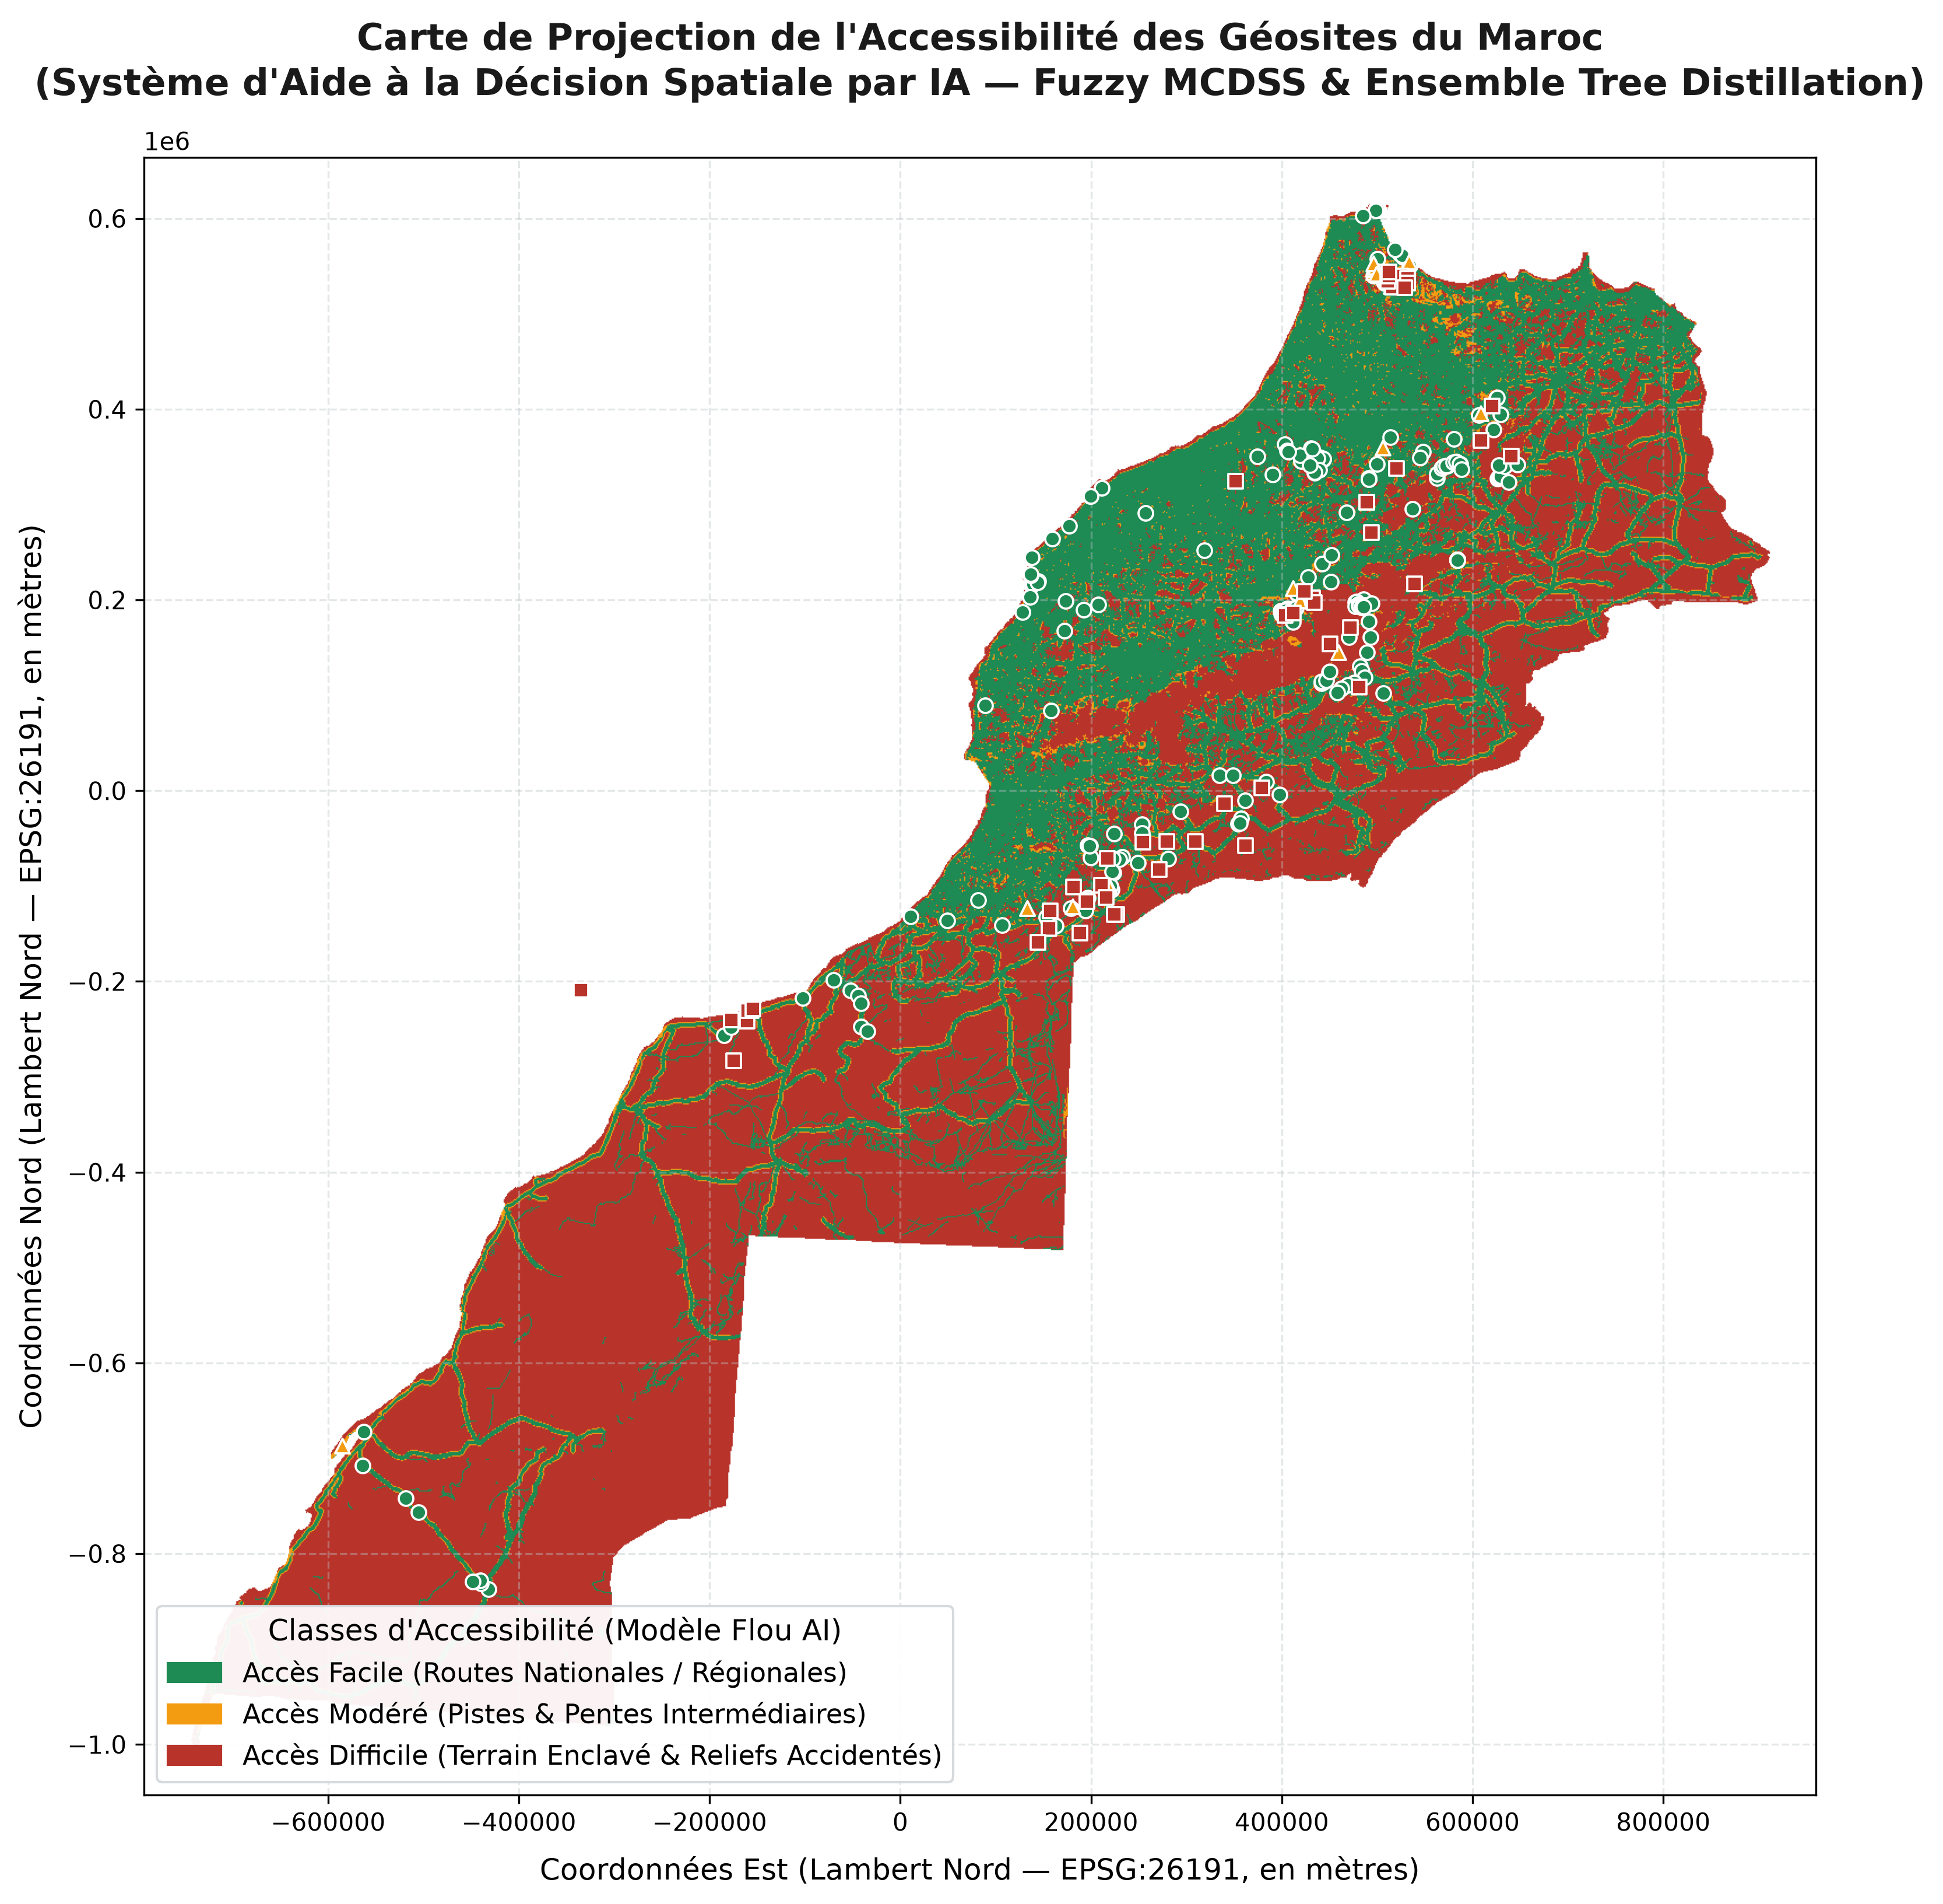
\includegraphics[width=0.9\textwidth]{../figures/morocco_fuzzy_mcdss_accessibility_map.png}
    \caption{Projected Continuous National Geosite Accessibility Map of Morocco (Fuzzy MCDSS AI Model).}
    \label{fig:map}
\end{figure*}

\section{Conclusions}
As an AI Research Intern at GSMI-UM6P, I (EL GORRIM Mohamed) have established a complete, end-to-end scientific pipeline that successfully scales geosite accessibility modeling to a national scale using a continuous Fuzzy MCDSS engine without border step artifacts. By introducing spatial block cross-validation and sigmoid membership functions, we resolved spatial leakage and artificial lowland penalization. The resulting nationwide dataset, saved models, and maps provide an essential tool for regional development, geotourism planning, and geological conservation.

\section*{Acknowledgments}
We thank the Geology and Sustainable Mining Institute (GSMI) and Mohammed VI Polytechnic University (UM6P) for providing the resources and datasets necessary to complete this project.

\begin{thebibliography}{1}
\bibitem{naimi2025}
M. Manaouch, L. Naimi, M. Haynou, M. Aghad, M. Sadiki, Q. B. Pham, and A. Jakimi, ``Enhancing Geotourism in Southeastern Morocco through Machine Learning-Based Geomorphosite Identification,'' \emph{Geoheritage}, vol. 17, no. 34, 2025.
\end{thebibliography}

\end{document}
